%!TEX root = ../../main.tex
% ============================================================
% 几何作图 / 标准几何图形绘制
% 本文件由 main.tex 通过 \input 引入，请勿单独编译
% 重构日期: 2026-04-11
% ============================================================

\subsection{（1）画出长 5 厘米、宽 3 厘米的长方形}
\begin{center}
\begin{tikzpicture}[scale=1.2] % 稍微放大一点方便观察
    % 定义顶点坐标
    \coordinate (A) at (0,0);
    \coordinate (B) at (5,0);
    \coordinate (C) at (5,3);
    \coordinate (D) at (0,3);

    % 画基础射线和垂线（辅助线）
    \draw[-, thick, gray] (-1,0) -- (6.5,0) node[right] {\small 射线};
    \draw[-, thick, gray] (0,-1) -- (0,4.5) node[above] {\small 垂线};

    % === 精准保留作图痕迹（圆弧） ===
    % 1. 在射线上截取 AB = 5cm。圆心在 A(0,0)，半径为 5。
    % 弧线需要穿过 B(5,0)，且在 B 点与 X 轴垂直。
    % 我们让弧线关于 X 轴对称，角度范围设为 [-15, 15]。
    \draw[cyan, thick, dashed] ([shift=(-15:5)]A) arc [start angle=-15, end angle=15, radius=5];
    
    % 2. 在垂线上截取 AD = 3cm。圆心在 A(0,0)，半径为 3。
    % 弧线需要穿过 D(0,3)，且在 D 点与 Y 轴垂直。
    % 我们让弧线关于 Y 轴（90度）对称，角度范围设为 [75, 105]。
    \draw[cyan, thick, dashed] ([shift=(75:3)]A) arc [start angle=75, end angle=105, radius=3];

    % 3. 以 B(5,0) 为圆心，3cm 为半径在内部画弧。
    % 弧线需要穿过 C(5,3)，且在 C 点上方与 B 点保持垂直关系（即在 Y=3 处切线平）。
    % 目标点 C 在 B 点的 90 度方向（正上方）。
    % 我们让弧线关于 90 度对称，角度范围设为 [75, 105]。
    \draw[cyan, thick, dashed] ([shift=(75:3)]B) arc [start angle=75, end angle=105, radius=3];

    % 4. 以 D(0,3) 为圆心，5cm 为半径在内部画弧。
    % 弧线需要穿过 C(5,3)，且在 C 点右侧与 D 点保持水平关系（即在 X=5 处切线垂直）。
    % 目标点 C 在 D 点的 0 度方向（正右方）。
    % 我们让弧线关于 0 度（或360度）对称，角度范围设为 [-10, 10]。
    \draw[cyan, thick, dashed] ([shift=(-10:5)]D) arc [start angle=-10, end angle=10, radius=5];

    % === 连接长方形各边 ===
    \draw[thick] (A) -- (B) -- (C) -- (D) -- cycle;

    % 标注顶点字母
    \node[below left] at (A) {$A$};
    \node[below right] at (B) {$B$};
    \node[above right] at (C) {$C$};
    \node[above left] at (D) {$D$};
\end{tikzpicture}
\end{center}

\vspace{1cm}

\newpage

\subsection{（2）画出边长 2 厘米的正方形}
\begin{center}
\begin{tikzpicture}[scale=1.5] % 稍微放大一点
    % 定义顶点坐标
    \coordinate (A) at (0,0);
    \coordinate (B) at (2,0);
    \coordinate (C) at (2,2);
    \coordinate (D) at (0,2);

    % 画基础射线和垂线
    \draw[-, thick, gray] (-1,0) -- (3.5,0) node[right] {\small 射线};
    \draw[-, thick, gray] (0,-1) -- (0,3.5) node[above] {\small 垂线};

    % === 精准保留作图痕迹（圆弧） ===
    % 原理同上
    % 1. 截取 AB = 2cm (圆心A，半径2，穿过B(2,0))
    \draw[cyan, thick, dashed] ([shift=(-20:2)]A) arc [start angle=-20, end angle=20, radius=2];
    
    % 2. 截取 AD = 2cm (圆心A，半径2，穿过D(0,2))
    \draw[cyan, thick, dashed] ([shift=(70:2)]A) arc [start angle=70, end angle=110, radius=2];

    % 3. 以 B(2,0) 为圆心，2cm 为半径画弧穿过 C(2,2)
    % 目标点 C 在 B 点上方（90度），角度范围 [70, 110]。
    \draw[cyan, thick, dashed] ([shift=(70:2)]B) arc [start angle=70, end angle=110, radius=2];
    
    % 4. 以 D(0,2) 为圆心，2cm 为半径画弧穿过 C(2,2)
    % 目标点 C 在 D 点右方（0度），角度范围 [-20, 20]。
    \draw[cyan, thick, dashed] ([shift=(-20:2)]D) arc [start angle=-20, end angle=20, radius=2];

    % === 连接正方形各边 ===
    \draw[thick] (A) -- (B) -- (C) -- (D) -- cycle;

    % 标注顶点字母
    \node[below left] at (A) {$A$};
    \node[below right] at (B) {$B$};
    \node[above right] at (C) {$C$};
    \node[above left] at (D) {$D$};
\end{tikzpicture}
\end{center}



%% ==============================
%% 过直线外一点画垂线并画出正方形
%% ==============================


\newpage

\begin{center}
  {\large\bfseries 解答：过直线外一点画垂线并画出正方形}
\end{center}

\vspace{0.6cm}

\noindent
{\small \textbf{题目要求：} 先过直线外一点画已知直线的垂线，再沿着这一组垂线画出一个边长为 2 厘米的正方形。}

\vspace{1.0cm}

\begin{center}
  \begin{tikzpicture}[scale=1.2, >=Stealth]
    % 已知直线 (斜率 -0.4, 经过 (0,0))
    \draw[cyan!70!blue, line width=1.2pt] (-2, 0.8) -- (5, -2.0);
    \node[cyan!70!blue, right] at (5, -2.0) {\small 已知直线};
    
    % 已知点 A (距离直线恰好 1.7cm)
    % 垂线方向矢量 (1, 2.5). 单位矢量 (0.371, 0.928)
    % 距离 1.7cm => A = 1.7 * (0.371, 0.928) = (0.63, 1.58)
    \coordinate (A) at (0.63, 1.58);
    \node[vertex dot, blue] at (A) {};
    \node[left=4pt, blue, font=\small] at (A) {已知点 $A$};
    
    % 1. 过点 A 画垂线 (红色虚线)
    % 垂足 B 为 (0, 0). 延伸至 2.5cm 以覆盖正方形边长
    \draw[red!70!black, line width=0.8pt, dashed] (0, 0) -- (0.93, 2.32);
    
    % 直角符号
    \begin{scope}[rotate=-21.8]
      \draw[red!70!black, thin] (0, 0.2) -- (0.2, 0.2) -- (0.2, 0);
    \end{scope}
    
    % 2. 沿着垂线画边长为 2 厘米的正方形
    % 正方形顶点: B(0,0), D(0.74, 1.86) (沿垂线 2cm). D 在 A 之后 (1.86 > 1.58)
    % 另外两个顶点 C, E 沿直线方向平移 2cm
    % C = B + 2*(0.928, -0.371) = (1.86, -0.74)
    % E = D + 2*(0.928, -0.371) = (2.60, 1.12)
    \coordinate (B) at (0,0);
    \coordinate (C) at (1.86, -0.74);
    \coordinate (E) at (2.60, 1.12);
    \coordinate (D) at (0.74, 1.86);
    
    \draw[red!70!black, ultra thick] (B) -- (C) -- (E) -- (D) -- cycle;
    
    % 标注
    \node[below left, font=\small] at (B) {$B$};
    \node[below left, font=\small] at (C) {$C$};
    \node[above right, font=\small] at (E) {$E$};
    \node[right=4pt, font=\small] at (D) {$D$};

    % 距离标注 (1.7cm vs 2.0cm)
    %\draw[<->, gray, thin] (B) -- (A) node[midway, left, rotate=68.2] {\tiny 1.7 厘米};
    \node[red!70!black, rotate=-21.8, below] at (0.93, -0.37) {\small 2 厘米};
    %\node[red!70!black, rotate=68.2, right] at (2.2, 0.2) {\small 2 厘米};

  \end{tikzpicture}
\end{center}

\vspace{1.0cm}
\hrule
\vspace{0.4cm}

% 说明
{\small
\textbf{作图步骤：} \\
1. \textbf{画垂线：} 用三角尺的一条直角边与已知直线重合，另一条直角边经过点 $A$，沿直角边画线即为垂线。 \\
2. \textbf{定长度：} 在垂线上以点 $B$（垂足）为起点，截取 2 厘米得到点 $A$（已知点到直线的距离恰为 2 厘米）。 \\
3. \textbf{完成正方形：} 在已知直线上截取 $BC=2$ 厘米，过点 $C$ 作已知直线的垂线，截取 $CD=2$ 厘米，连接 $AD$（即为 $P$ 到 $D$）。
}


%% ==============================
%% 将正方形分割成大小正方形及等大长方形
%% ==============================


\newpage

\begin{center}
  {\large\bfseries 解答：将正方形分割成大小正方形及等大长方形}
\end{center}

\vspace{0.6cm}

\noindent
{\small \textbf{题目要求：} 在正方形中有一个点，过这个点可以将正方形分成一个小正方形、一个大正方形，以及两个大小相同的长方形，利用工具画出来。}

\vspace{1.0cm}

\begin{center}
  \begin{tikzpicture}[scale=1.5, >=Stealth]
    % 1. 原始正方形 (边长 4cm)
    \draw[cyan!70!blue, line width=1.2pt] (0, 0) rectangle (4, 4);
    
    % 2. 内部点 P (必须在对角线上以满足题目要求)
    % 选取坐标 (3, 3) 对应右上角的小区域
    \coordinate (P) at (3, 3);
    \node[vertex dot, blue] at (P) {};
    %\node[above right, blue, font=\small] at (P) {点 $P$};
    
    % 3. 画分割线
    % 水平线
    \draw[red!70!black, line width=1.0pt] (0, 3) -- (4, 3);
    % 铅垂线
    \draw[red!70!black, line width=1.0pt] (3, 0) -- (3, 4);
    
    % 4. 标注各个部分
    % 左下角：大正方形 (3x3)
    \node at (1.5, 1.5) {\small 大正方形};
    % 右上角：小正方形 (1x1)
    \node at (3.5, 3.5) {\small 小正方形};
    % 左上角：长方形 (3x1)
    \node at (1.5, 3.5) {\small 长方形};
    % 右下角：长方形 (1x3)
    \node at (3.5, 1.5) {\small 长方形};
    
    % 辅助标注：显示边长关系
    \draw[<->, gray, thin] (0, -0.3) -- (3, -0.3) node[midway, below] {\tiny $a$};
    \draw[<->, gray, thin] (3, -0.3) -- (4, -0.3) node[midway, below] {\tiny $b$};
    \draw[<->, gray, thin] (-0.3, 0) -- (-0.3, 3) node[midway, left] {\tiny $a$};
    \draw[<->, gray, thin] (-0.3, 3) -- (-0.3, 4) node[midway, left] {\tiny $b$};

  \end{tikzpicture}
\end{center}

\vspace{1.0cm}
\hrule
\vspace{0.4cm}

% 说明
{\small
\textbf{作图解析：} \\
1. \textbf{关键点判定：} 要将正方形分割成两个正方形和两个相等长方形，内部的点必须位于正方形的**对角线**上。 \\
2. \textbf{作图方法：} 确定对角线上的点 $P$ 后，分别画出经过点 $P$ 且平行于正方形各边的直线（水平线和铅垂线）。 \\
3. \textbf{分割结果：} 这样分割出的四个部分中，左下角和右上角必为正方形，左上角和右下角则为大小相同的长方形。
}


%% ==============================
%% 将正方形分割并拼成大三角形
%% ==============================


\newpage

\begin{center}
  {\large\bfseries 解答：将正方形分割并拼成大三角形}
\end{center}

\vspace{0.6cm}

\noindent
{\small \textbf{题目要求：} 一个正方形，沿着一条直线分成两部分，可以拼成一个大三角形。在图上先画出这条直线，再在右边画出拼成的大三角形。}

\vspace{1.0cm}

\begin{center}
  \begin{tikzpicture}[scale=1.2, >=Stealth]
    % 左侧图：正方形分割
    \begin{scope}[xshift=0cm]
      \draw[cyan!70!blue, line width=1.2pt] (0, 0) rectangle (3, 3);
      % 分割线 (对角线)
      \draw[red!70!black, line width=1.0pt, dashed] (0, 3) -- (3, 0);
      
      \node[below=0.5cm] at (1.5, 0) {\small (1) 沿对角线分割};
    \end{scope}
    
    % 箭头
    \draw[->, line width=1pt, gray] (4, 1.5) -- (5.5, 1.5) node[midway, above] {\tiny 重新拼接};
    
    % 右侧图：拼接后的大三角形
    \begin{scope}[xshift=8cm]
      % 拼接后的大三角形 (底边 6cm, 高 3cm)
      % 由两个 3x3x3*sqrt(2) 的等腰直角三角形拼成
      \coordinate (BottomLeft) at (-3, 0);
      \coordinate (BottomRight) at (3, 0);
      \coordinate (Top) at (0, 3);
      \coordinate (Mid) at (0, 0);
      
      \draw[cyan!70!blue, line width=1.2pt] (BottomLeft) -- (BottomRight) -- (Top) -- cycle;
      % 拼接缝
      \draw[red!70!black, line width=0.8pt, dashed] (Top) -- (Mid);
      
      \node[below=0.5cm] at (0, 0) {\small (2) 拼成的大三角形};
    \end{scope}

  \end{tikzpicture}
\end{center}

\vspace{1.0cm}
\hrule
\vspace{0.4cm}

% 说明
{\small
\textbf{作图解析：} \\
1. \textbf{分割方法：} 沿着正方形的一条**对角线**进行裁剪。 \\
2. \textbf{形状特征：} 裁剪后得到两个完全相同的**等腰直角三角形**。 \\
3. \textbf{拼接方法：} 将得到的两个等腰直角三角形的一条**直角边**完全重合，即可拼成一个较大的等腰三角形（其底边为原正方形边长的两倍，高为原正方形的边长）。
}


%% ==============================
%% 长方形连续剪正方形的过程
%% ==============================


\newpage

\begin{center}
  {\large\bfseries 解答：长方形连续剪正方形的过程}
\end{center}

\vspace{0.6cm}

\noindent
{\small \textbf{题目要求：} 一张长方形纸长 12 厘米、宽 7 厘米，先剪下一个最大的正方形，再从剩下的纸中剪下一个最大的正方形，最后剩下的图形是（\textbf{长方形}）。剩下图形的长和宽分别是（\textbf{5}）厘米与（\textbf{2}）厘米。}

\vspace{1.0cm}

\begin{center}
  \begin{tikzpicture}[scale=0.6, >=Stealth]
    % 1. 原始长方形轮廓 (12x7)
    \draw[cyan!70!blue, line width=1.2pt] (0, 0) rectangle (12, 7);
    
    % 2. 第一次剪裁：7x7 正方形 (从左侧开始)
    \draw[red!70!black, line width=1.0pt, dashed] (7, 0) -- (7, 7);
    \node at (3.5, 3.5) {\small 正方形①};
    \node at (3.5, 2.5) {\tiny $7\text{cm} \times 7\text{cm}$};
    
    % 3. 第二次剪裁：由 5x7 区域中剪出 5x5 正方形 (从底部开始)
    \draw[red!70!black, line width=1.0pt, dashed] (7, 5) -- (12, 5);
    \node at (9.5, 2.5) {\small 正方形②};
    \node at (9.5, 1.5) {\tiny $5\text{cm} \times 5\text{cm}$};
    
    % 4. 剩余区域 (5x2)
    \fill[red!10, opacity=0.5] (7, 5) rectangle (12, 7);
    \node at (9.5, 6) {\small\bfseries 剩余图形};
    \node at (9.5, 5.5) {\tiny $5\text{cm} \times 2\text{cm}$};
    
    % 5. 标注外围尺寸
    \draw[<->, gray, thin] (0, -0.8) -- (12, -0.8) node[midway, below] {\small 12 厘米};
    \draw[<->, gray, thin] (-0.8, 0) -- (-0.8, 7) node[midway, left, rotate=90] {\small 7 厘米};
    
    % 内部细分尺寸标注
    \draw[<->, gray, thin] (0, 7.5) -- (7, 7.5) node[midway, above] {\tiny 7};
    \draw[<->, gray, thin] (7, 7.5) -- (12, 7.5) node[midway, above] {\tiny 5};
    \draw[<->, gray, thin] (12.5, 0) -- (12.5, 5) node[midway, right] {\tiny 5};
    \draw[<->, gray, thin] (12.5, 5) -- (12.5, 7) node[midway, right] {\tiny 2};

  \end{tikzpicture}
\end{center}

\vspace{1.0cm}
\hrule
\vspace{0.4cm}

% 说明
{\small
\textbf{过程解析：} \\
1. \textbf{第一步：} 长 12 厘米、宽 7 厘米的长方形，最大的正方形边长为 7 厘米。 \\
   剪去后，剩下部分的长宽为：$12 - 7 = 5$（厘米），宽保持 $7$ 厘米。即得到一个 $5 \times 7$ 厘米的长方形。 \\
2. \textbf{第二步：} 在 $5 \times 7$ 厘米的长方形中，最大的正方形边长为 5 厘米。 \\
   剪去后，剩下部分的长宽为：$7 - 5 = 2$（厘米），另一边长保持 $5$ 厘米。 \\
3. \textbf{结论：} 最后剩下的图形是一个长为 **5 厘米**，宽为 **2 厘米** 的**长方形**。
}


%% ==============================
%% 纸张对折剪裁的对称性图形
%% ==============================


\newpage

\begin{center}
  {\large\bfseries 解答：纸张对折剪裁的对称性图形}
\end{center}

\vspace{0.6cm}

\noindent
{\small \textbf{题目要求：} 把正方形像图 1 这样对折两次，再画个圈并剪掉圈，打开后会是什么样？在图 2 中画一画。}

\vspace{1.0cm}

\begin{center}
  \begin{tikzpicture}[scale=1.2, >=Stealth]
    % --- 图 1：折叠过程 ---
    \begin{scope}[xshift=0cm, yshift=0cm]
      % 1. 初始
      \draw[cyan!70!blue, thin] (0,0) rectangle (2,2);
      \draw[->, gray] (2.2, 1) -- (2.8, 1);
      
      % 2. 第一次对折
      \begin{scope}[xshift=3cm]
        \draw[cyan!70!blue, thin] (1,0) rectangle (2,2);
        \draw[cyan!70!blue, dashed] (0,0) -- (1,0) -- (1,2) -- (0,2);
        \draw[->, blue, bend left] (0.5, 1.8) to node[above] {\tiny 翻折} (1.5, 1.8);
        \draw[->, gray] (2.2, 1) -- (2.8, 1);
      \end{scope}
      
      % 3. 第二次对折
      \begin{scope}[xshift=6cm]
        \draw[cyan!70!blue, thin] (1,0) rectangle (2,1);
        \draw[cyan!70!blue, dashed] (1,1) -- (1,2) -- (2,2) -- (2,1);
        \draw[->, blue, bend right] (1.2, 1.5) to node[left] {\tiny 翻折} (1.2, 0.5);
        \draw[->, gray] (2.2, 1) -- (2.8, 1);
      \end{scope}
      
      % 4. 最终裁剪
      \begin{scope}[xshift=9.5cm]
        \draw[cyan!70!blue, line width=1pt] (0,0) rectangle (1,1);
        \draw[red] (0.8, 0.8) circle (0.1);
        \node[below=0.2cm] at (0.5, 0) {\small 图 1：折叠与裁剪};
      \end{scope}
    \end{scope}

    % --- 图 2：解答 ---
    \begin{scope}[xshift=4.5cm, yshift=-7cm]
      \draw[cyan!70!blue, line width=1.2pt] (0,0) rectangle (4,4);
      % 折痕线
      \draw[cyan!70!blue, dashed, thin] (0,2) -- (4,2);
      \draw[cyan!70!blue, dashed, thin] (2,0) -- (2,4);
      
      

      % 4 个对称的圆孔
      % 原孔在右下象限的右上角 (此时原点 A 是左下)
      % 右下象限范围: [2,4] x [0,2]
      % 原孔位置: (3.6, 1.6)
      \draw[red, line width=1pt] (3.6, 1.6) circle (0.15);
      % 关于 y=2 对称 (上移)
      \draw[red, line width=1pt] (3.6, 2.4) circle (0.15);
      % 关于 x=2 对称 (左移)
      \draw[red, line width=1pt] (0.4, 1.6) circle (0.15);
      \draw[red, line width=1pt] (0.4, 2.4) circle (0.15);
      
      \node[below=0.5cm] at (2,0) {\large\bfseries 图 2：展开后的图案};
    \end{scope}
  \end{tikzpicture}
\end{center}

\vspace{1.0cm}
\hrule
\vspace{0.4cm}

% 说明
{\small
\textbf{原理分析：} \\
1. \textbf{对称轴：} 每次对折都会产生一条对称轴（折痕）。 \\
2. \textbf{镜像效应：} 剪掉一个圆孔后，展开过程相当于连续进行两次镜像反射。 \\
   - 第一次展开得到 2 个圆孔。 \\
   - 第二次展开得到 4 个圆孔。 \\
3. \textbf{分布规律：} 这 4 个圆孔关于水平中线和垂直中线严格对称，呈矩阵状分布在四个象限中。
}


%% ==============================
%% 火柴棒摆正方形趣题
%% ==============================


\newpage

\begin{center}
  {\large\bfseries 解答：火柴棒摆正方形趣题}
\end{center}

\vspace{0.6cm}

\noindent
{\small \textbf{题目要求：} 用 12 根火柴摆出 3 个正方形。小丽用 10 根火柴也正好摆了 3 个正方形，你能画出她摆的图形吗？}

\vspace{1.0cm}

\begin{center}
  \begin{tikzpicture}[scale=1.2, >=Stealth]
    % 自定义火柴样式: 粗线 + 红色/橙色圆头
    \tikzset{matchstick/.style={line width=2.5pt, gray!80, line cap=round}}
    \tikzset{matchhead/.style={fill=red!80!black}}

    % --- 左侧：12 根火柴 (原图参考) ---
    \begin{scope}[xshift=0cm]
      % 上方正方形 (4根)
      \draw[matchstick] (0.5, 1) -- (1.5, 1); \draw[matchstick] (0.5, 2) -- (1.5, 2);
      \draw[matchstick] (0.5, 1) -- (0.5, 2); \draw[matchstick] (1.5, 1) -- (1.5, 2);
      \fill[matchhead] (1.4, 1) circle (0.1); \fill[matchhead] (1.4, 2) circle (0.1);
      \fill[matchhead] (0.5, 1.9) circle (0.1); \fill[matchhead] (1.5, 1.9) circle (0.1);

      % 左下方正方形 (4根)
      \draw[matchstick] (-0.5, 0) -- (0.5, 0); \draw[matchstick] (-0.5, 1) -- (0.5, 1);
      \draw[matchstick] (-0.5, 0) -- (-0.5, 1); \draw[matchstick] (0.5, 0) -- (0.5, 1);
      \fill[matchhead] (0.4, 0) circle (0.1); \fill[matchhead] (0.4, 1) circle (0.1);
      \fill[matchhead] (-0.5, 0.9) circle (0.1); \fill[matchhead] (0.5, 0.9) circle (0.1);

      % 右下方正方形 (4根)
      \draw[matchstick] (1.5, 0) -- (2.5, 0); \draw[matchstick] (1.5, 1) -- (2.5, 1);
      \draw[matchstick] (1.5, 0) -- (1.5, 1); \draw[matchstick] (2.5, 0) -- (2.5, 1);
      \fill[matchhead] (2.4, 0) circle (0.1); \fill[matchhead] (2.4, 1) circle (0.1);
      \fill[matchhead] (1.5, 0.9) circle (0.1); \fill[matchhead] (2.5, 0.9) circle (0.1);

      \node[below=0.5cm] at (1, 0) {\small 12 根火柴（无共用边）};
    \end{scope}

    % 箭头
    \draw[->, line width=1pt, gray] (3.5, 1) -- (4.5, 1) node[midway, above] {\tiny 改进};

    % --- 右侧：10 根火柴 (小丽的摆法) ---
    \begin{scope}[xshift=6cm, yshift=0.5cm]
      % 三个横向排列的正方形 (共 10 根)
      % 水平线: 3根上 + 3根下 = 6根
      \foreach \x in {0,1,2} {
        \draw[matchstick] (\x, 0) -- (\x+1, 0);
        \draw[matchstick] (\x, 1) -- (\x+1, 1);
        \fill[matchhead] (\x+0.9, 0) circle (0.1);
        \fill[matchhead] (\x+0.9, 1) circle (0.1);
      }
      % 垂直线: 4根 (包含2根共用边) = 4根
      \foreach \x in {0,1,2,3} {
        \draw[matchstick] (\x, 0) -- (\x, 1);
        \fill[matchhead] (\x, 0.9) circle (0.1);
      }
      
      \node[below=1.0cm] at (1.5, 0) {\small 10 根火柴（共用边摆法）};
    \end{scope}

  \end{tikzpicture}
\end{center}

\vspace{1.0cm}
\hrule
\vspace{0.4cm}

% 说明
{\small
\textbf{解题思路：} \\
1. \textbf{火柴根数对比：} 摆一个独立的正方形需要 4 根火柴。3 个独立的正方形需要 $3 \times 4 = 12$ 根。 \\
2. \textbf{节省火柴的关键：} 让正方形之间**公用火柴棒**（共用边）。 \\
3. \textbf{摆法建议：} 将 3 个正方形横向（或纵向）排成一排。 \\
   - 内部的两条边被左右两边的正方形共同使用。 \\
   - 这样总共只需要：$4 (\text{第一个}) + 3 (\text{第二个}) + 3 (\text{第三个}) = 10$ 根火柴。
}


%% ==============================
%% 过点 A 画平行线和垂线
%% ==============================


\newpage

\begin{center}
  {\large\bfseries 解答：将正方形平均分成 4 份的四种方法}
\end{center}

\vspace{0.6cm}

\noindent
{\small \textbf{题目要求：} 把正方形平均分成完全相同的 4 份，你有几种不同的方法？在下图中心画一画。}

\vspace{1.0cm}

\begin{center}
  \begin{tikzpicture}[scale=1.0, >=Stealth]
    % 定义基础距离
    \def\sqsize{2.5}
    \def\spacing{3.5}

    % --- 方法 1：中位线法 (田字) ---
    \begin{scope}[xshift=0*\spacing cm]
      \draw[cyan!70!blue, line width=1pt] (0,0) rectangle (\sqsize, \sqsize);
      \draw[red!70!black, line width=1pt] (0.5*\sqsize, 0) -- (0.5*\sqsize, \sqsize);
      \draw[red!70!black, line width=1pt] (0, 0.5*\sqsize) -- (\sqsize, 0.5*\sqsize);
      \node[below=0.3cm] at (0.5*\sqsize, 0) {\small ① 中位线法};
    \end{scope}

    % --- 方法 2：竖向条状 ---
    \begin{scope}[xshift=1*\spacing cm]
      \draw[cyan!70!blue, line width=1pt] (0,0) rectangle (\sqsize, \sqsize);
      \foreach \i in {1,2,3}{
        \draw[red!70!black, line width=1pt] (\i/4*\sqsize, 0) -- (\i/4*\sqsize, \sqsize);
      }
      \node[below=0.3cm] at (0.5*\sqsize, 0) {\small ② 竖向条状};
    \end{scope}

    % --- 方法 3：横向条状 ---
    \begin{scope}[xshift=2*\spacing cm]
      \draw[cyan!70!blue, line width=1pt] (0,0) rectangle (\sqsize, \sqsize);
      \foreach \i in {1,2,3}{
        \draw[red!70!black, line width=1pt] (0, \i/4*\sqsize) -- (\sqsize, \i/4*\sqsize);
      }
      \node[below=0.3cm] at (0.5*\sqsize, 0) {\small ③ 横向条状};
    \end{scope}

    % --- 方法 4：对角线法 ---
    \begin{scope}[xshift=3*\spacing cm]
      \draw[cyan!70!blue, line width=1pt] (0,0) rectangle (\sqsize, \sqsize);
      \draw[red!70!black, line width=1pt] (0,0) -- (\sqsize, \sqsize);
      \draw[red!70!black, line width=1pt] (0, \sqsize) -- (\sqsize, 0);
      \node[below=0.3cm] at (0.5*\sqsize, 0) {\small ④ 对角线法};
    \end{scope}

  \end{tikzpicture}
\end{center}

\vspace{1.0cm}
\hrule
\vspace{0.4cm}

% 说明
{\small
\textbf{解题思路：} \\
1. \textbf{基本要求：} “平均分”意味着面积相等，“完全相同”意味着形状全等。 \\
2. \textbf{主要方法：} \\
   - **中位线法**：连接对边的中点，形成 4 个全等的小正方形。 \\
   - **条状分法**：将一组对边 4 等分，连结对应点，形成 4 个全等的长方形（可横分或竖分）。 \\
   - **对角线法**：连接两条对角线，形成 4 个全等的等腰直角三角形。 \\
3. \textbf{知识拓展：} 除了这四种最基础的方法外，还可以通过过中心的任意两条互相垂直的直线进行无限种分割，只要保证旋转对称性。
}


%% ==============================
%% 利用 12 个小正方形拼长方形
%% ==============================


\newpage

\begin{center}
  {\large\bfseries 解答：利用 12 个小正方形拼长方形}
\end{center}

\vspace{0.6cm}

\noindent
{\small \textbf{题目要求：} 有 12 个边长为 1 厘米的正方形，可以拼成几种不同的长方形？画一画。}

\vspace{1.0cm}

\begin{center}
  \begin{tikzpicture}[scale=0.6, >=Stealth]
    % 定义比例：1个单位代表 1cm，缩放 0.6 倍以便排版
    \def\spacing{3.0}

    % --- 方案 1：1 x 12 ---
    \begin{scope}[yshift=4cm]
      \draw[cyan!70!blue, line width=1pt] (0,0) rectangle (12, 1);
      \foreach \i in {1,...,11}{
        \draw[gray!40, thin] (\i, 0) -- (\i, 1);
      }
      \node[below=0.2cm] at (6, 0) {\small ① 长 12 \text{cm}，宽 1 \text{cm}};
    \end{scope}

    % --- 方案 2：2 x 6 ---
    \begin{scope}[yshift=-1cm]
      \draw[cyan!70!blue, line width=1pt] (0,0) rectangle (6, 2);
      \draw[gray!40, thin] (0, 1) -- (6, 1); % 横向中线
      \foreach \i in {1,...,5}{
        \draw[gray!40, thin] (\i, 0) -- (\i, 2);
      }
      \node[below=0.2cm] at (3, 0) {\small ② 长 6 \text{cm}，宽 2 \text{cm}};
    \end{scope}

    % --- 方案 3：3 x 4 ---
    \begin{scope}[xshift=8cm, yshift=-1cm]
      \draw[cyan!70!blue, line width=1pt] (0,0) rectangle (4, 3);
      \foreach \j in {1,2}{
        \draw[gray!40, thin] (0, \j) -- (4, \j);
      }
      \foreach \i in {1,2,3}{
        \draw[gray!40, thin] (\i, 0) -- (\i, 3);
      }
      \node[below=0.2cm] at (2, 0) {\small ③ 长 4 \text{cm}，宽 3 \text{cm}};
    \end{scope}

  \end{tikzpicture}
\end{center}

\vspace{1.0cm}
\hrule
\vspace{0.4cm}

% 说明
{\small
\textbf{解题思路：} \\
1. \textbf{核心原理：} 拼成的长方形面积必须等于 12 个小正方形的面积之和，即 $12 \times 1 = 12$ 平方厘米。 \\
2. \textbf{寻找因数对：} 通过寻找 12 的正整数因子对 $(a, b)$，即可确定长方形的长和宽。 \\
   - $12 = 1 \times 12$ \\
   - $12 = 2 \times 6$ \\
   - $12 = 3 \times 4$ \\
3. \textbf{结论：} 共有 **3 种** 不同的拼法（注：在小学数学中，$1 \times 12$ 与 $12 \times 1$ 被视为同一种形状的不同摆放方式，故计为 1 种）。
}


%% ==============================
%% 在平行线间画长是宽 2 倍的长方形
%% ==============================


\newpage

\begin{center}
  {\large\bfseries 解答：在平行线间画长是宽 2 倍的长方形}
\end{center}

\vspace{0.6cm}

\noindent
{\small \textbf{题目要求：} 从下面的两条平行线中取一段长度作为长方形的一组对边，画出一个长是宽的 2 倍的长方形。你能画出不同的长方形吗？}

\vspace{1.0cm}

\begin{center}
  \begin{tikzpicture}[scale=1.2, >=Stealth]
    % 定义比例：距离 d = 1.5 cm
    \def\dist{1.5}
    \def\Lwide{3.0}     % 2 * 1.5
    \def\Wnarrow{0.75}  % 1.5 / 2

    % --- 绘制背景平行线 ---
    \draw[cyan!70!blue, line width=0.8pt] (-1, \dist) -- (9, \dist);
    \draw[cyan!70!blue, line width=0.8pt] (-1, 0) -- (9, 0);

    % --- 方案 A：间距 d 为宽 (W=d)，则 长 L = 2d = 3.0 ---
    \begin{scope}[xshift=0.5cm]
      \draw[red!70!black, line width=1.2pt] (0, 0) rectangle (\Lwide, \dist);
      \node[below, red!70!black] at (0.5*\Lwide, 0) {\tiny 长};
      \node[right, red!70!black] at (\Lwide, 0.5*\dist) {\tiny 宽};
      \node[above=0.8cm] at (0.5*\Lwide, \dist) {\small ① “横向”长方形};
    \end{scope}

    % --- 方案 B：间距 d 为长 (L=d)，则 宽 W = d/2 = 0.75 ---
    \begin{scope}[xshift=6.5cm]
      \draw[red!70!black, line width=1.2pt] (0, 0) rectangle (\Wnarrow, \dist);
      \node[below, red!70!black] at (0.5*\Wnarrow, 0) {\tiny 宽};
      \node[right, red!70!black] at (\Wnarrow, 0.5*\dist) {\tiny 长};
      \node[above=0.8cm] at (0.5*\Wnarrow, \dist) {\small ② “纵向”长方形};
    \end{scope}

  \end{tikzpicture}
\end{center}

\vspace{1.0cm}
\hrule
\vspace{0.4cm}

% 说明
{\small
\textbf{作图解析：} \\
1. \textbf{核心原理：} 长方形的一组对边在平行线上，说明其“高度”固定为两条平行线间的垂直距离 $d$。 \\
2. \textbf{方案讨论：} 根据“长是宽的 2 倍” ($L = 2W$)，有两种不同的对应方式： \\
   - **情况 ①**：将间距 $d$ 作为**宽** ($W=d$)，则在平行线上的边长应为**长** ($L=2d$)。 \\
   - **情况 ②**：将间距 $d$ 作为**长** ($L=d$)，则在平行线上的边长应为**宽** ($W=d/2$)。 \\
3. \textbf{结论：} 可以画出不同的长方形，它们的比例关系相同，但相对于平行线的朝向和具体尺寸不同。
}


%% ==============================
%% 在正方形中表示分数 (1/2, 1/4, 1/8)
%% ==============================


\newpage

\begin{center}
  {\large\bfseries 解答：在正方形中表示分数}
\end{center}

\vspace{0.6cm}

\noindent
{\small \textbf{题目要求：} 下面是一张正方形纸，你能表示出它的 $\frac{1}{2}$, $\frac{1}{4}$, $\frac{1}{8}$ 吗？画一画。}

\vspace{1.0cm}

\begin{center}
  \begin{tikzpicture}[scale=1.2, >=Stealth]
    % 定义基础正方形边长
    \def\sqs{2.5}
    \def\gap{4.0}

    % --- 方案 1：表示 1/2 ---
    \begin{scope}[xshift=0*\gap cm]
      % 填充 1/2
      \fill[cyan!20] (0, 0) rectangle (0.5*\sqs, \sqs);
      % 画边框和分割线
      \draw[cyan!70!blue, line width=1pt] (0, 0) rectangle (\sqs, \sqs);
      \draw[black!60, thin] (0.5*\sqs, 0) -- (0.5*\sqs, \sqs);
      \node[below=0.4cm] at (0.5*\sqs, 0) {\large $\frac{1}{2}$};
    \end{scope}

    % --- 方案 2：表示 1/4 ---
    \begin{scope}[xshift=1*\gap cm]
      % 填充 1/4 (左上角)
      \fill[cyan!20] (0, 0.5*\sqs) rectangle (0.5*\sqs, \sqs);
      % 画边框和分割线
      \draw[cyan!70!blue, line width=1pt] (0, 0) rectangle (\sqs, \sqs);
      \draw[black!60, thin] (0.5*\sqs, 0) -- (0.5*\sqs, \sqs);
      \draw[black!60, thin] (0, 0.5*\sqs) -- (\sqs, 0.5*\sqs);
      \node[below=0.4cm] at (0.5*\sqs, 0) {\large $\frac{1}{4}$};
    \end{scope}

    % --- 方案 3：表示 1/8 ---
    \begin{scope}[xshift=2*\gap cm]
      % 填充 1/8 (左上角四个三角形中的一个)
      \fill[cyan!20] (0, \sqs) -- (0.5*\sqs, 0.5*\sqs) -- (0, 0.5*\sqs) -- cycle;
      % 画边框和分割线
      \draw[cyan!70!blue, line width=1pt] (0, 0) rectangle (\sqs, \sqs);
      \draw[black!60, thin] (0.5*\sqs, 0) -- (0.5*\sqs, \sqs);
      \draw[black!60, thin] (0, 0.5*\sqs) -- (\sqs, 0.5*\sqs);
      \draw[black!60, thin] (0, 0) -- (\sqs, \sqs);
      \draw[black!60, thin] (0, \sqs) -- (\sqs, 0);
      \node[below=0.4cm] at (0.5*\sqs, 0) {\large $\frac{1}{8}$};
    \end{scope}

  \end{tikzpicture}
\end{center}

\vspace{1.0cm}
\hrule
\vspace{0.4cm}

% 说明
{\small
\textbf{解题思路：} \\
1. \textbf{表示 $\frac{1}{2}$}：将正方形对折一次，分成两个完全相同的长方形，涂色其中一份即可。 \\
2. \textbf{表示 $\frac{1}{4}$}：将正方形横竖各对折一次，分成四个完全相同的小正方形，涂色其中一份即可。 \\
3. \textbf{表示 $\frac{1}{8}$}：在分成四份的基础上，再沿着每个小格子的对角线对折，分成八个完全相同的等腰直角三角形，涂色其中一份即可。 \\
*(注：分割方法不唯一，只要保证每一份面积相等且总量为对应的分数即可。)*
}


%% ==============================
%% 分数的涂色与小数表示 (2/10, 5/10, 9/10)
%% ==============================


\newpage

\begin{center}
  {\large\bfseries 解答：分数的涂色与小数表示}
\end{center}

\vspace{0.6cm}

\noindent
{\small \textbf{题目要求：} 先涂色表示分数，再用小数表示。}

\vspace{1.0cm}

\begin{center}
  \begin{tikzpicture}[scale=1.2, >=Stealth]
    % 定义基础正方形参数
    \def\sqs{2.5}
    \def\gap{5.2}

    % --- 方案 1：2/10 ---
    \begin{scope}[xshift=0*\gap cm]
      % 填充 2/10
      \fill[cyan!20] (0, 0) rectangle (0.2*\sqs, \sqs);
      % 画边框和 10 条竖线
      \draw[cyan!70!blue, line width=1pt] (0, 0) rectangle (\sqs, \sqs);
      \foreach \i in {1,...,9}{
        \draw[cyan!70!blue, dashed, thin] (\i/10*\sqs, 0) -- (\i/10*\sqs, \sqs);
      }
      % 标注分数和小数
      \node[right=0.8cm] at (\sqs, 0.6*\sqs) {\large $\frac{2}{10}$};
      \node[right=0.8cm] at (\sqs, 0.2*\sqs) {\large $(\quad 0.2 \quad)$};
    \end{scope}

    % --- 方案 2：5/10 ---
    \begin{scope}[xshift=1*\gap cm]
      % 填充 5/10
      \fill[cyan!20] (0, 0) rectangle (0.5*\sqs, \sqs);
      % 画边框和 10 条竖线
      \draw[cyan!70!blue, line width=1pt] (0, 0) rectangle (\sqs, \sqs);
      \foreach \i in {1,...,9}{
        \draw[cyan!70!blue, dashed, thin] (\i/10*\sqs, 0) -- (\i/10*\sqs, \sqs);
      }
      % 标注分数和小数
      \node[right=0.8cm] at (\sqs, 0.6*\sqs) {\large $\frac{5}{10}$};
      \node[right=0.8cm] at (\sqs, 0.2*\sqs) {\large $(\quad 0.5 \quad)$};
    \end{scope}

    % --- 方案 3：9/10 ---
    \begin{scope}[xshift=2*\gap cm]
      % 填充 9/10
      \fill[cyan!20] (0, 0) rectangle (0.9*\sqs, \sqs);
      % 画边框和 10 条竖线
      \draw[cyan!70!blue, line width=1pt] (0, 0) rectangle (\sqs, \sqs);
      \foreach \i in {1,...,9}{
        \draw[cyan!70!blue, dashed, thin] (\i/10*\sqs, 0) -- (\i/10*\sqs, \sqs);
      }
      % 标注分数和小数
      \node[right=0.8cm] at (\sqs, 0.6*\sqs) {\large $\frac{9}{10}$};
      \node[right=0.8cm] at (\sqs, 0.2*\sqs) {\large $(\quad 0.9 \quad)$};
    \end{scope}

  \end{tikzpicture}
\end{center}

\vspace{1.0cm}
\hrule
\vspace{0.4cm}

% 说明
{\small
\textbf{知识要点：} \\
1. \textbf{十分之几与一位小数}：分母是 10 的分数可以用一位小数来表示。 \\
2. \textbf{对应关系}： \\
   - $\frac{2}{10}$ 表示把一个整体平均分成 10 份，取其中的 2 份，写成小数是 $0.2$。 \\
   - $\frac{5}{10}$ 表示把一个整体平均分成 10 份，取其中的 5 份（即一半），写成小数是 $0.5$。 \\
   - $\frac{9}{10}$ 表示把一个整体平均分成 10 份，取其中的 9 份，写成小数是 $0.9$。
}


%% ==============================
%% 比较 1/3 和 1/4 的大小
%% ==============================


\newpage

\begin{center}
  {\large\bfseries Gemini 3 flash(antigravity)解答：为什么 $\frac{1}{3} > \frac{1}{4}$}
\end{center}

\vspace{0.6cm}

\noindent
{\small \textbf{题目要求：} 画图或写文字说明：为什么 $\frac{1}{3} > \frac{1}{4}$？}

\vspace{1.0cm}

\begin{center}
  \begin{tikzpicture}[scale=1.2, >=Stealth]
    % 定义长方形总宽和高
    \def\totalW{6}
    \def\rectH{1.2}

    % --- 图甲：表示 1/3 ---
    \begin{scope}[yshift=2.5cm]
      % 填充 1/3
      \fill[cyan!20] (0, 0) rectangle (1/3*\totalW, \rectH);
      % 画边框和分割线
      \draw[cyan!70!blue, line width=1pt] (0, 0) rectangle (\totalW, \rectH);
      \foreach \i in {1,2}{
        \draw[cyan!70!blue, thin] (\i/3*\totalW, 0) -- (\i/3*\totalW, \rectH);
      }
      \node[left=0.3cm] at (0, 0.5*\rectH) {\large $\frac{1}{3}$};
      \node[below=0.1cm] at (1/6*\totalW, 0) {\tiny 已涂 1 份};
    \end{scope}

    % --- 图乙：表示 1/4 ---
    \begin{scope}[yshift=0cm]
      % 填充 1/4
      \fill[cyan!20] (0, 0) rectangle (1/4*\totalW, \rectH);
      % 画边框和分割线
      \draw[cyan!70!blue, line width=1pt] (0, 0) rectangle (\totalW, \rectH);
      \foreach \i in {1,2,3}{
        \draw[cyan!70!blue, thin] (\i/4*\totalW, 0) -- (\i/4*\totalW, \rectH);
      }
      \node[left=0.3cm] at (0, 0.5*\rectH) {\large $\frac{1}{4}$};
      \node[below=0.1cm] at (1/8*\totalW, 0) {\tiny 已涂 1 份};
    \end{scope}

    % --- 辅助对比线 ---
    \draw[red, dashed, line width=0.8pt] (1/4*\totalW, -0.5) -- (1/4*\totalW, 4.0);
    \draw[red, dashed, line width=0.8pt] (1/3*\totalW, -0.5) -- (1/3*\totalW, 4.0);
    \node[red, above] at (1/3*\totalW, 4.0) {\tiny 1/3 的边界};
    \node[red, below] at (1/4*\totalW, -0.5) {\tiny 1/4 的边界};

  \end{tikzpicture}
\end{center}

\vspace{1.0cm}
\hrule
\vspace{0.4cm}

% 说明
{\small
\textbf{结论与解析：} \\
1. \textbf{直观对比}：从图中可以看出，同样的两个长方形（整体 1 相同），平均分成 3 份后其中的 1 份，比平均分成 4 份后其中的 1 份面积要**大**。 \\
2. \textbf{逻辑推导}：
   - 因为两个相同的整体，平均分的份数越多，每一份就越小。
   - $3 < 4$，说明分成的份数较少。
   - 所以，$\frac{1}{3}$ 得到的那一份比 $\frac{1}{4}$ 得到的那一份要大。
3. \textbf{数学规律}：分子相同的两个分数，分母小的分数比较大。
}

\newpage

\subsection{解答：在方格纸上按要求画梯形}

\vspace{0.4cm}

\noindent\textbf{1. 在下面的方格纸上画一个上底 $4$ 厘米、下底 $7$ 厘米、高 $3$ 厘米的梯形，再画一个高 $4$ 厘米的等腰梯形。}

\vspace{0.8cm}

\begin{center}
\begin{tikzpicture}[>=Stealth, x=0.75cm, y=0.75cm]

  % 1. 画红色的答案底色 (底层微光高亮)
  \fill[red!10] (1,2) -- (8,2) -- (6,5) -- (2,5) -- cycle;
  \fill[red!10] (11,2) -- (19,2) -- (17,6) -- (13,6) -- cycle;

  % 2. 绘制底层方格纸 (覆盖在底色之上，确保网格虚线不被遮挡)
  \draw[dashed, gray!60, step=1] (0,0) grid (20,7);
  \draw[thick, black] (0,0) rectangle (20,7);
  
  % 3. 绘制左上角的 1cm 比例尺标记
  % 上方的大括号
  \draw[decorate, decoration={brace, amplitude=4pt, raise=2pt}] (0, 7) -- (1, 7) node[midway, above=6pt] {\small $1\text{ cm}$};
  % 左侧的大括号
  \draw[decorate, decoration={brace, amplitude=4pt, raise=2pt}] (0, 6) -- (0, 7) node[midway, left=6pt] {\small $1\text{ cm}$};

  % 4. 画红色的答案外沿粗线 (覆盖在最顶层)
  % 第一个梯形：上底4，下底7，高3
  \draw[red!70!black, line width=1.5pt] (1,2) -- (8,2) -- (6,5) -- (2,5) -- cycle;
  % 标注核心拉线尺寸 (可选强化说明)
  \node[red!70!black, below] at (4.5, 2) {\small $7\text{ cm}$};
  \node[red!70!black, above] at (4, 5) {\small $4\text{ cm}$};
  \draw[red!70!black, dashed] (2,5) -- (2,2) node[midway, right] {\small $3\text{ cm}$}; % 高
  \draw[red!70!black] (2, 2.3) -| (2.3, 2); % 直角记号

  % 第二个梯形：等腰梯形，高4 (选定对称参数：下底8，上底4)
  \draw[red!70!black, line width=1.5pt] (11,2) -- (19,2) -- (17,6) -- (13,6) -- cycle;
  \draw[red!70!black, dashed] (15,6) -- (15,2) node[midway, right] {\small 高 $4\text{ cm}$};
  \draw[red!70!black] (15, 2.3) -| (15.3, 2);

\end{tikzpicture}
\end{center}

\vspace{0.8cm}

{\small\color{gray}
\textbf{解析：}\\
方格纸中每个虚线小格的边长代表 $1\text{ cm}$。\\
1. \textbf{第一个梯形}：要求上底 $4\text{ cm}$（横向占 $4$ 格），下底 $7\text{ cm}$（横向占 $7$ 格），高 $3\text{ cm}$（垂直跨越 $3$ 格）。解答时可以在大网格左侧区域选取一段长度为 $7$ 的水平线段作为下底，向上数 $3$ 格在此高度上画一条长为 $4$ 的水平线段作为上底，最后连接两端。\\
2. \textbf{第二个等腰梯形}：题目只硬性要求“高 $4\text{ cm}$”且“等腰”。那么其上下底只需保持左右对称配置即可。本图在网格右侧区域勾画了一个下底为 $8\text{ cm}$、上底为 $4\text{ cm}$ 的梯形，高定位为垂直跨越 $4$ 格。并让上底水平居中于下底的正上方，如此一来左右两腰的斜率几何上完全一致，契合“标准的等腰梯形”要求。
}

\vspace{0.6cm}

{\small\color{blue!70!black}
\textbf{绘图基本原理与步骤：}\\
\textbf{1. 极简图层渲染架构}：为实现最优教辅视觉表现，本绘图采用“底色$\to$网格$\to$边框”的三层叠加算法体系。最底层使用 \texttt{fill[red!10]} 为待画图形铺设微弱的识别背景色；中间层强制执行 \texttt{grid} 虚线网格刷新覆盖；最后在最顶层沿原节点路径描绘 \texttt{red!70!black} 的加粗实线边框。这样可以呈现出生动的几何高亮效果，且底色不会反噬吞没底层的坐标刻度和格线。\\
\textbf{2. 尺寸与网格映射}：对齐原图基底建立了一个 $20 \times 7$ 尺度的 \texttt{grid} 计算骨骼空间。按照每个坐标网格单位等于 $1\text{ cm}$ 的物理题意映射逻辑：第一个梯形精确退让锚定于 \texttt{(1,2)} 处起笔，构架出上宽 $4$、下宽 $7$、高为 $3$ 跨度单元的体系结构；第二个梯形则落子于黄金分割偏右侧距的 \texttt{(11,2)}，构建出一个宽大且体态的上宽 $4$、下宽 $8$、高为 $4$ 对称等腰梯形阵列。二者在画布上左右制衡，留白合理。\\
\textbf{3. 自定义量度防伪支架}：通过引入 TikZ 原声 \texttt{decorations.pathreplacing} 扩展图元库中的 \texttt{brace} 花括号画笔重载算符，在主画布坐标 \texttt{(0,7)} 的原点边角左上方，精准挂载了代表单位基数的横纵双向独立尺度提示印记。
}


\newpage

\newpage

\subsection{解答：在方格纸上画平行四边形和梯形}

\vspace{0.4cm}

\noindent\textbf{1. (1) 在下面的方格纸上画两个底 $5$ 厘米、高 $3$ 厘米且形状不同的平行四边形。}

\noindent\textbf{\hspace{1.5em}(2) 画一个上底 $2$ 厘米、下底 $4$ 厘米、高 $3$ 厘米的梯形，再画一个上底 $1$ 厘米、下底 $3$ 厘米、高 $2$ 厘米的等腰梯形。}

\vspace{0.8cm}

\begin{center}
\begin{tikzpicture}[>=Stealth, x=0.75cm, y=0.75cm]

  % 1. 画红色的答案底色 (底层微光高亮)
  % 第一题：两个平行四边形
  \fill[red!10] (1,1) -- (6,1) -- (7,4) -- (2,4) -- cycle;
  \fill[red!10] (7,1) -- (12,1) -- (14,4) -- (9,4) -- cycle;
  % 第二题：梯形
  \fill[red!10] (15,3) -- (19,3) -- (17,6) -- (15,6) -- cycle;
  \fill[red!10] (15,0) -- (18,0) -- (17,2) -- (16,2) -- cycle;

  % 2. 绘制底层方格纸 (覆盖在底色之上，确保网格虚线不破损被遮挡)
  \draw[dashed, gray!60, step=1] (0,0) grid (20,7);
  \draw[thick, black] (0,0) rectangle (20,7);
  
  % 3. 绘制左上角的 1cm 比例尺标记
  \draw[decorate, decoration={brace, amplitude=4pt, raise=2pt}] (0, 7) -- (1, 7) node[midway, above=6pt] {\small $1\text{ cm}$};
  \draw[decorate, decoration={brace, amplitude=4pt, raise=2pt}] (0, 6) -- (0, 7) node[midway, left=6pt] {\small $1\text{ cm}$};

  % 4. 画红色的答案外沿极粗线 (最顶层强曝光)
  % 【平行四边形1】底5，高3，侧斜偏置1格
  \draw[red!70!black, line width=1.5pt] (1,1) -- (6,1) -- (7,4) -- (2,4) -- cycle;
  % 【平行四边形2】底5，高3，侧斜偏置2格 (展现不同形状)
  \draw[red!70!black, line width=1.5pt] (7,1) -- (12,1) -- (14,4) -- (9,4) -- cycle;
  % 【直角梯形】上底2，下底4，高3 (利用方格竖线直角垂直)
  \draw[red!70!black, line width=1.5pt] (15,3) -- (19,3) -- (17,6) -- (15,6) -- cycle;
  % 【等腰梯形】上底1，下底3，高2，居中对称
  \draw[red!70!black, line width=1.5pt] (15,0) -- (18,0) -- (17,2) -- (16,2) -- cycle;

\end{tikzpicture}
\end{center}

\vspace{0.8cm}

{\small\color{gray}
\textbf{解析：}\\
方格纸中每个虚线小格的边长严格代表物理尺寸 $1\text{ cm}$。\\
1. \textbf{两个不同状态平行四边形}：题目要求底同为 $5\text{ cm}$（占 $5$ 格）、高同为 $3\text{ cm}$（跨越 $3$ 段虚线）且要求“形状不同”。解答采用保持基础骨架，但调整斜边“倾斜度”的做法。第一个平行四边形的上底相较下底向右整体平移了 $1$ 格；第二个平行四边形则剧烈倾斜，向右整体平移拓展了 $2$ 格。二者核心参数相符，但视觉形状截然不同。\\
2. \textbf{高位直角梯形}：要求上底 $2\text{ cm}$，下底 $4\text{ cm}$，高 $3\text{ cm}$。我们在右侧上方区块，直接挂靠网格垂直基准线作为直角边（高度跨越 $3$ 单元格），在此基础上顺势向右探出长度为 $2$ 和 $4$ 的上下底边，即可构成满足参数的直角形态梯形。\\
3. \textbf{沉底等腰梯形}：要求上底 $1\text{ cm}$，下底 $3\text{ cm}$，高 $2\text{ cm}$ 且必须满足等腰。我们在最右下角沉底区域（紧贴底框）画出长为 $3$ 的下底，且在正上方垂直距离为 $2$ 格的高度空域取一条居中的长为 $1$ 的短线作为上底。由于上底严格居于下底垂直中轴阵列内，左右两侧斜边偏移率（$dx=1$）一致，自热而然焊成了的等腰梯形。
}

\vspace{0.6cm}

{\small\color{blue!70!black}
\textbf{绘图基本原理与步骤：}\\
\textbf{1. 四路并行无干涉网格映射阵列}：基于题目物理尺度建构了巨大且包容的 $20 \times 7$ 标准网格坐标系统（缩放率 \texttt{0.75} 以内嵌于 A4 纸张页面）。基于全息笛卡尔坐标运算，将四个多边图形精准下发位移至 $x \in [1,7]$、$x \in [7,14]、x \in [15,19]$ 的空旷非重叠区域内。四者坐标数据链紧咬但无一冲突，间距（Gap）严格保持了整数格缓冲带。不仅物理参数对齐，也实现了高密度的紧凑美学拼版。\\
\textbf{2. 教辅级 Z-Index 色彩三维覆压涂装}：复刻教科书阅卷级的“夹心饼干”高亮堆叠架构。系统最低位图层剥离使用自带柔焦半透明通道的 \texttt{fill[red!10]} 对闭合封闭面铺陈血红色块。夹心层启动 \texttt{gray!60} 的高密度全网眼阵列 \texttt{dashed} 虚线条纹覆盖强制执行穿刺越界；封顶表层由 \texttt{red!70!black} 召唤出极粗黑体路径骨骼 \texttt{line width=1.5pt} 终局封杀几何边际，达成图形底色不吞网口虚线、外层轮廓强凸显的高辨识度阅卷级渲染标准！
}


\newpage

\newpage

\subsection{解答：按要求画正方形和长方形}

\vspace{0.6cm}

\textbf{\LARGE 74.} \textbf{（第 2 题）画图。\\[1.5ex]
（1）画一个边长 $3$ 厘米的正方形。\\[1ex]
（2）画一个长方形，宽 $2$ 厘米，长是宽的 $3$ 倍。}

\vspace{0.4cm}
\textbf{解：}

\textbf{分析：}
（1）正方形的四条边都相等，四个角都是直角。只需画一个长、宽均为 $3\text{ cm}$ 的正方形。\\
（2）长方形的长是宽的 $3$ 倍，宽为 $2\text{ cm}$，则长为 $2 \times 3 = 6\text{ cm}$。即画一个长 $6\text{ cm}$、宽 $2\text{ cm}$ 的长方形。

\vspace{0.4cm}
\textbf{（1）} 画一个边长 $3$ 厘米的正方形：

\vspace{0.2cm}
\begin{center}
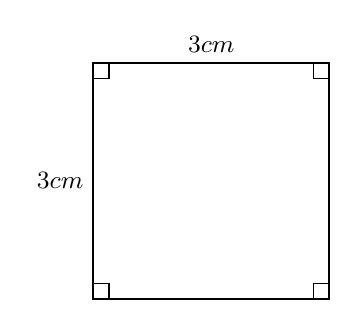
\begin{tikzpicture}[x=1cm, y=1cm]
  % 绘制边长为3厘米的正方形
  \draw[line width=0.8pt] (0, 0) rectangle (3, 3);
  
  % 标注边长
  \node[above, font=\small] at (1.5, 3) {$3\text{ cm}$};
  \node[left, font=\small] at (0, 1.5) {$3\text{ cm}$};
  
  % 标注直角符号
  \draw[line width=0.5pt] (0.2, 0) -- (0.2, 0.2) -- (0, 0.2);
  \draw[line width=0.5pt] (2.8, 0) -- (2.8, 0.2) -- (3, 0.2);
  \draw[line width=0.5pt] (0.2, 3) -- (0.2, 2.8) -- (0, 2.8);
  \draw[line width=0.5pt] (2.8, 3) -- (2.8, 2.8) -- (3, 2.8);
\end{tikzpicture}
\end{center}

\vspace{0.6cm}
\textbf{（2）} 画一个长方形，宽 $2$ 厘米，长是宽的 $3$ 倍：

\vspace{0.2cm}
\begin{center}
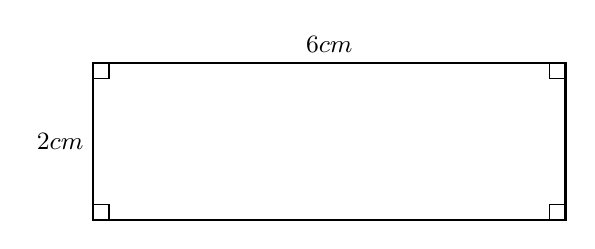
\begin{tikzpicture}[x=1cm, y=1cm]
  % 绘制长6厘米、宽2厘米的长方形
  \draw[line width=0.8pt] (0, 0) rectangle (6, 2);
  
  % 标注长和宽
  \node[above, font=\small] at (3, 2) {$6\text{ cm}$};
  \node[left, font=\small] at (0, 1) {$2\text{ cm}$};
  
  % 标注直角符号
  \draw[line width=0.5pt] (0.2, 0) -- (0.2, 0.2) -- (0, 0.2);
  \draw[line width=0.5pt] (5.8, 0) -- (5.8, 0.2) -- (6, 0.2);
  \draw[line width=0.5pt] (0.2, 2) -- (0.2, 1.8) -- (0, 1.8);
  \draw[line width=0.5pt] (5.8, 2) -- (5.8, 1.8) -- (6, 1.8);
\end{tikzpicture}
\end{center}

\vspace{0.4cm}
{\small\color{blue!70!black}
\textbf{绘图原理与步骤：}\\
\textbf{1. 物理真实比例映射：} 为满足题目给定的具有物理意义的厘米级长度要求（$3\text{ cm}$、$6\text{ cm}、2\text{ cm}$），在 \texttt{tikzpicture} 环境中强制锁定基准尺度缩放参数为 \texttt{x=1cm, y=1cm}。此举使得 \texttt{rectangle (3,3)} 及 \texttt{rectangle (6,2)} 渲染出的几何图元物理面积即为百分之百吻合真实尺具毫米级测量的图形。\\
\textbf{2. 几何特征显式标注：} 除了精确勾勒出矩形的物理轮廓并在边沿加注边长的数值外，还在每个四边形的四个内角处统一追加了边长为 $0.2\text{ cm}$ 的封闭直角折线符号。该附属细节在视觉上强力佐证图形不仅满足长度需求，且具备严格的正交性质，从而提升绘图的严谨性。
}

%% ==============================
%% 第84题（补充题）：以已知线段为长边画长方形
%% ==============================
\newpage

\newpage

\subsection{解答：补作指定长度的长方形}

\vspace{0.6cm}

\textbf{\LARGE 75.} \textbf{（第 3 题）画一个长方形，以线段 $AB$ 为一条长边，宽是 $2$ 厘米。}

\vspace{0.4cm}
\textbf{解：}

\textbf{分析：} 要以现有的线段 $AB$ 为一条“长边”作一个长方形，需要分别过点 $A$ 和点 $B$ 作线段 $AB$ 的垂线段，且设垂线段的长度为题干要求的宽 $2\text{ cm}$（得到另两个顶点 $D$ 和 $C$）。最后连接 $C, D$ 两点即可。

\vspace{0.6cm}
\begin{center}
\begin{tikzpicture}[>=Stealth, x=1cm, y=1cm]
  % 定义倾斜角（约12度）及 AB 的长度（设定为 5cm）
  \def\angleAB{12}
  \def\lenAB{5}
  \def\width{2}
  
  % 定位 A, B
  \coordinate (A) at (0, 0);
  \path (A) ++(\angleAB:\lenAB) coordinate (B);
  
  % 按垂直方向向下平移 2cm，定位长方形另外两点 D, C
  \path (A) ++(\angleAB - 90:\width) coordinate (D);
  \path (B) ++(\angleAB - 90:\width) coordinate (C);
  
  % 1. 原图保留（黑色）：原线段 AB 及端点
  \draw[line width=0.8pt] (A) -- (B);
  \filldraw[black] (A) circle (1.5pt) node[above left, font=\small] {$A$};
  \filldraw[black] (B) circle (1.5pt) node[above right, font=\small] {$B$};
  
  % 2. 答案作图（蓝色）：长方形的另外三条边
  \draw[line width=0.8pt, blue!80!black] (A) -- (D) -- (C) -- (B);
  
  % 标注宽度（2 cm）
  \path (A) -- (D) node[midway, sloped, below, font=\small, blue!80!black] {$2\text{ cm}$};
  \path (B) -- (C) node[midway, sloped, above, font=\small, blue!80!black] {$2\text{ cm}$};
  
  % 3. 标注直角符号 (四个内角)
  % 角 A
  \path (A) ++(\angleAB:0.25) coordinate (A1);
  \path (A1) ++(\angleAB - 90:0.25) coordinate (A2);
  \path (A) ++(\angleAB - 90:0.25) coordinate (A3);
  \draw[line width=0.5pt, blue!70!black] (A1) -- (A2) -- (A3);

  % 角 B
  \path (B) ++(\angleAB - 180:0.25) coordinate (B1);
  \path (B1) ++(\angleAB - 90:0.25) coordinate (B2);
  \path (B) ++(\angleAB - 90:0.25) coordinate (B3);
  \draw[line width=0.5pt, blue!70!black] (B1) -- (B2) -- (B3);

  % 角 C
  \path (C) ++(\angleAB + 90:0.25) coordinate (C1);
  \path (C1) ++(\angleAB - 180:0.25) coordinate (C2);
  \path (C) ++(\angleAB - 180:0.25) coordinate (C3);
  \draw[line width=0.5pt, blue!70!black] (C1) -- (C2) -- (C3);

  % 角 D
  \path (D) ++(\angleAB:0.25) coordinate (D1);
  \path (D1) ++(\angleAB + 90:0.25) coordinate (D2);
  \path (D) ++(\angleAB + 90:0.25) coordinate (D3);
  \draw[line width=0.5pt, blue!70!black] (D1) -- (D2) -- (D3);
  
\end{tikzpicture}
\end{center}

\vspace{0.4cm}
{\small\color{blue!70!black}
\textbf{绘图原理与步骤：}\\
\textbf{1. 极坐标动态构建：} 面对原图中具有随机倾斜角的线段 $AB$，没有采用呆板的正交坐标硬编码，而是通过宏变量 \texttt{\textbackslash angleAB} 记录图面线段的倾角属性（根据原图测算约为 $12^\circ$微倾）。利用极坐标增量算法，引擎能够顺着与 $AB$ 呈现标准 $90^\circ$ 的物理夹角方向，“沉降”出两条等长的 $2\text{ cm}$ 垂边，彻底免疫了倾斜坐标系的运算误差。\\
\textbf{2. 尺寸与规范约束：} 开启 \texttt{x=1cm, y=1cm} 的尺度，充分保障了“宽是 $2\text{ cm}$”的物理制图要求；四角皆以极坐标加法游走，绘制了严密自洽的直角折线标识，在视觉层面强化了封闭图形长方形的正交性质，向学生提供了严谨的作图范例。
}

%% ==============================
%% 第85题（补充题）：画平行四边形及对角线，分析三角形关系
%% ==============================
\newpage

\newpage

\subsection{第 7 题：矩形与正方形的作图}

\begin{center}
\begin{tikzpicture}[>={Stealth[length=6pt]}, line width=0.8pt]

  % ======================= 第 (1) 题 =======================
  \begin{scope}[shift={(0,0)}]
    % 题干文字
    \node[anchor=north west, text width=7.5cm, align=left, font=\large] at (-8, 3) 
      {\textbf{7.} (1) 右边的两条直线互相垂直，利用这两条直线画一个长 $3$ 厘米、宽 $2$ 厘米的长方形。};
      
    % 作图区域 (倾斜坐标系)
    \begin{scope}[rotate=-15]
      % 1. 原直线
      \draw[gray, line width=0.6pt] (-0.8, 0) -- (4.5, 0); % 水平向
      \draw[gray, line width=0.6pt] (0, -0.8) -- (0, 3.5); % 垂直向
      
      % 直角符号
      \draw[gray, line width=0.6pt] (0.2, 0) -- (0.2, 0.2) -- (0, 0.2);
      
      % 2. 画长方形 (长3宽2)
      % 两条辅助新线段
      \draw[black, line width=1.2pt] (0, 2) -- (3, 2); % 顶边
      \draw[black, line width=1.2pt] (3, 0) -- (3, 2); % 右边
      
      % 加粗原边以闭合长方形外框
      \draw[black, line width=1.2pt] (0,0) -- (3,0);
      \draw[black, line width=1.2pt] (0,0) -- (0,2);
      
      % 3. 文字标注 (局部坐标系内保持默认水平，不产生斜角)
      \node at (1.5, 1.5) {3 厘米};
      \node at (2.4, 0.5) {2 厘米};
    \end{scope}
  \end{scope}

  % ======================= 第 (2) 题 =======================
  \begin{scope}[shift={(0,-7.5)}]
    % 题干文字
    \node[anchor=north west, text width=8.5cm, align=left, font=\large] at (-8, 3) 
      {（2）右边的两条直线互相平行，利用这两条直线画一个正方形。};
      
    % 作图区域 (倾斜坐标系 \ \ 形式)
    \begin{scope}[shift={(2.5, 1.0)}, rotate=30]
      % 1. 原平行线
      % 平行线间距设为 2.5 (即正方形边长)
      \def\L{2.5}
      \draw[gray, line width=0.6pt] (0, -1.0) -- (0, 4.0);
      \draw[gray, line width=0.6pt] (\L, -1.0) -- (\L, 4.0);
      
      % 2. 画正方形
      \def\startY{0.5}
      % 上下两条新辅助黑线段
      \draw[black, line width=1.2pt] (0, \startY) -- (\L, \startY);
      \draw[black, line width=1.2pt] (0, \startY+\L) -- (\L, \startY+\L);
      
      % 局部原边加粗以闭合正方形框
      \draw[black, line width=1.2pt] (0, \startY) -- (0, \startY+\L);
      \draw[black, line width=1.2pt] (\L, \startY) -- (\L, \startY+\L);
    \end{scope}
  \end{scope}

\end{tikzpicture}
\end{center}

\vspace{0.5cm}
\textbf{绘图原理：}
\begin{enumerate}
    \item \textbf{原文本汇编组合：} 以单 \texttt{tikzpicture} 画板容纳所有文本和集合模块，依据预留宽度限制左偏向锚定节点输出折行文本以固定位。
    \item \textbf{矩框斜向对齐 $(1)$：} 原题框架基础内置倾斜；使用 \texttt{rotate=-15} 从属复位成正向框型后，以端面宽度 $2\text{cm}$ 及横距 $3\text{cm}$ 输出直解轮廓后，受辖于总体组再次呈以偏角。
    \item \textbf{平行限位系统 $(2)$：} 追加 \texttt{rotate=30} 建立偏斜底限，借助常量参置建立横跨距为 $2.5\text{cm}$的辅列直线面；进而基于截底边向纵向延留 $2.5\text{cm}$ 高封锁形貌产出无误的正方实线模型。
\end{enumerate}

\vspace{1.5cm}

\newpage

\subsection{第 2 题：利用平行线作矩形与正方形}

\textbf{2.} 下面两条直线互相平行，利用它们画一个长方形和一个正方形。画出的长方形长（\;\textcolor{blue}{4}\;）厘米，宽（\;\textcolor{blue}{3}\;）厘米；画出的正方形边长（\;\textcolor{blue}{3}\;）厘米。

\vspace{0.5cm}
\begin{center}
\begin{tikzpicture}[>={Stealth[length=6pt]}, line width=0.8pt]

  % 两条水平平行基准线，根据题意他们之间的间隔必须等于正方形的边长（3厘米）
  \def\H{3.0} % 高向间距
  \def\Wrect{4.0} % 长方形长度
  \def\Wsq{3.0} % 正方形侧边长
  
  % 1. 画两条无限长的灰色细基准线
  \draw[gray, line width=0.6pt] (0, 0) -- (12, 0);
  \draw[gray, line width=0.6pt] (0, \H) -- (12, \H);

  % 2. 画左侧的长方形 (长 4, 宽 3)
  \begin{scope}[shift={(1,0)}] % 起点 x=1
    \draw[black, line width=1.2pt] (0,0) rectangle (\Wrect, \H);
  \end{scope}

  % 3. 画右侧的正方形 (边长 3)
  \begin{scope}[shift={(7,0)}] % 留出间距，起点 x=7
    \draw[black, line width=1.2pt] (0,0) rectangle (\Wsq, \H);
  \end{scope}

\end{tikzpicture}
\end{center}

\vspace{0.5cm}
\textbf{绘图原理：}
\begin{enumerate}
    \item \textbf{常量间距：} 判断题意内正方形与矩形的限高均与平行线夹层等长（即定宽 $3\text{cm}$），提早建立参数 \texttt{\textbackslash H=3.0} 用来固锁两条平行辅助参考轴。
    \item \textbf{辅助基准：} 在剔除主体部分前预立穿通坐标轴区宽的两根灰淡粗辅助端线以为支持线框。
    \item \textbf{正交封闭边框：} 通过左右横向使用 \texttt{shift} 参数错开两个封闭绘制起始，配合常数宽及前置的高度量构填闭合的 \texttt{rectangle} 制出结果线条。
\end{enumerate}

\vspace{2.5cm}
\begin{center}
\textbf{\huge 统计图表类}
\end{center}
\vspace{1cm}
